\section{Processi di supporto}
\subsection{Documentazione}
\subsubsection{Attività}
\paragraph{Documentazione} 
Il gruppo di lavoro \GRUPPO\ si impegna a registrare tutte le informazioni acquisite nel corso del ciclo di vita\G\ del \textit{software} all'interno di una serie ben definita di documenti descritti in questa sezione. Nello specifico, vengono spiegati gli standard da rispettare per la stesura dei documenti e i passaggi necessari per renderli formalmente corretti.

\subsubsection{Procedure}
\paragraph{Gestione dei documenti}
La stesura di un nuovo documento viene decisa dal \textit{Responsabile di Progetto}. Tutta la documentazione deve essere creata attraverso l'uso di un \textit{template}\G\ \LaTeX\ disponibile nel \textit{repository}\G\ GitHub\G\ del gruppo, al fine di mantenerne uniforme la struttura e lo stile.

\paragraph{Creazione di un nuovo documento}
Nel \textit{repository}\G\ è presente un \textit{file} generico denonimato \textit{new\_doc.tex} contenente un \textit{template} adattabile ad ogni nuovo documento. Il \textit{file} deve essere incluso con il \textit{template} \LaTeX\, che è messo a disposizione di tutti i membri del gruppo. Ogni redattore deve possedere tutti i \textit{file} previsti dal \textit{template} al fine di creare correttamente un nuovo documento.

\paragraph{Avanzamento di un documento}
La procedura adottata per sviluppare un documento è la seguente ed è riportata in \hyperref[sec:Figura3]{Figura 3}:
\begin{itemize}
	\item [1.] Il \textit{Responsabile di Progetto} si preoccupa di assegnare la stesura del documento a uno o più redattori, a seconda della complessità dello stesso. L'assegnazione è gestita attraverso \textit{task}\G\ organizzati tramite il servizio \textit{online} Teamwork\G; 
	\item [2.] A stesura completata, ogni assegnatario ha il compito di etichettare il \textit{task} come completato;
	\item [3.] Il \textit{Verificatore} riceve in automatico un'email che segnala il completamento del documento;
	\item [4.] Nel caso si riscontrassero errori durante la fase di verifica, il \textit{Verificatore} deve occuparsi di creare un nuovo \textit{task} da assegnare al redattore del documento;
	\item [5.] Nel caso di documento corretto, il \textit{Verificatore} deve completare il \textit{task} assegnatogli. Un'email viene quindi automaticamente recapitata al \textit{Responsabile di Progetto}.
	\item [6.] Il \textit{Responsabile di Progetto} deve infine approvare il documento. In caso di mancata approvazione, il \textit{Verificatore} deve creare un nuovo \textit{task} indirizzato al redattore, che si occuperà di correggere gli errori in base alle segnalazioni emesse. 
\end{itemize}

\begin{figure}[htbp]
\centering
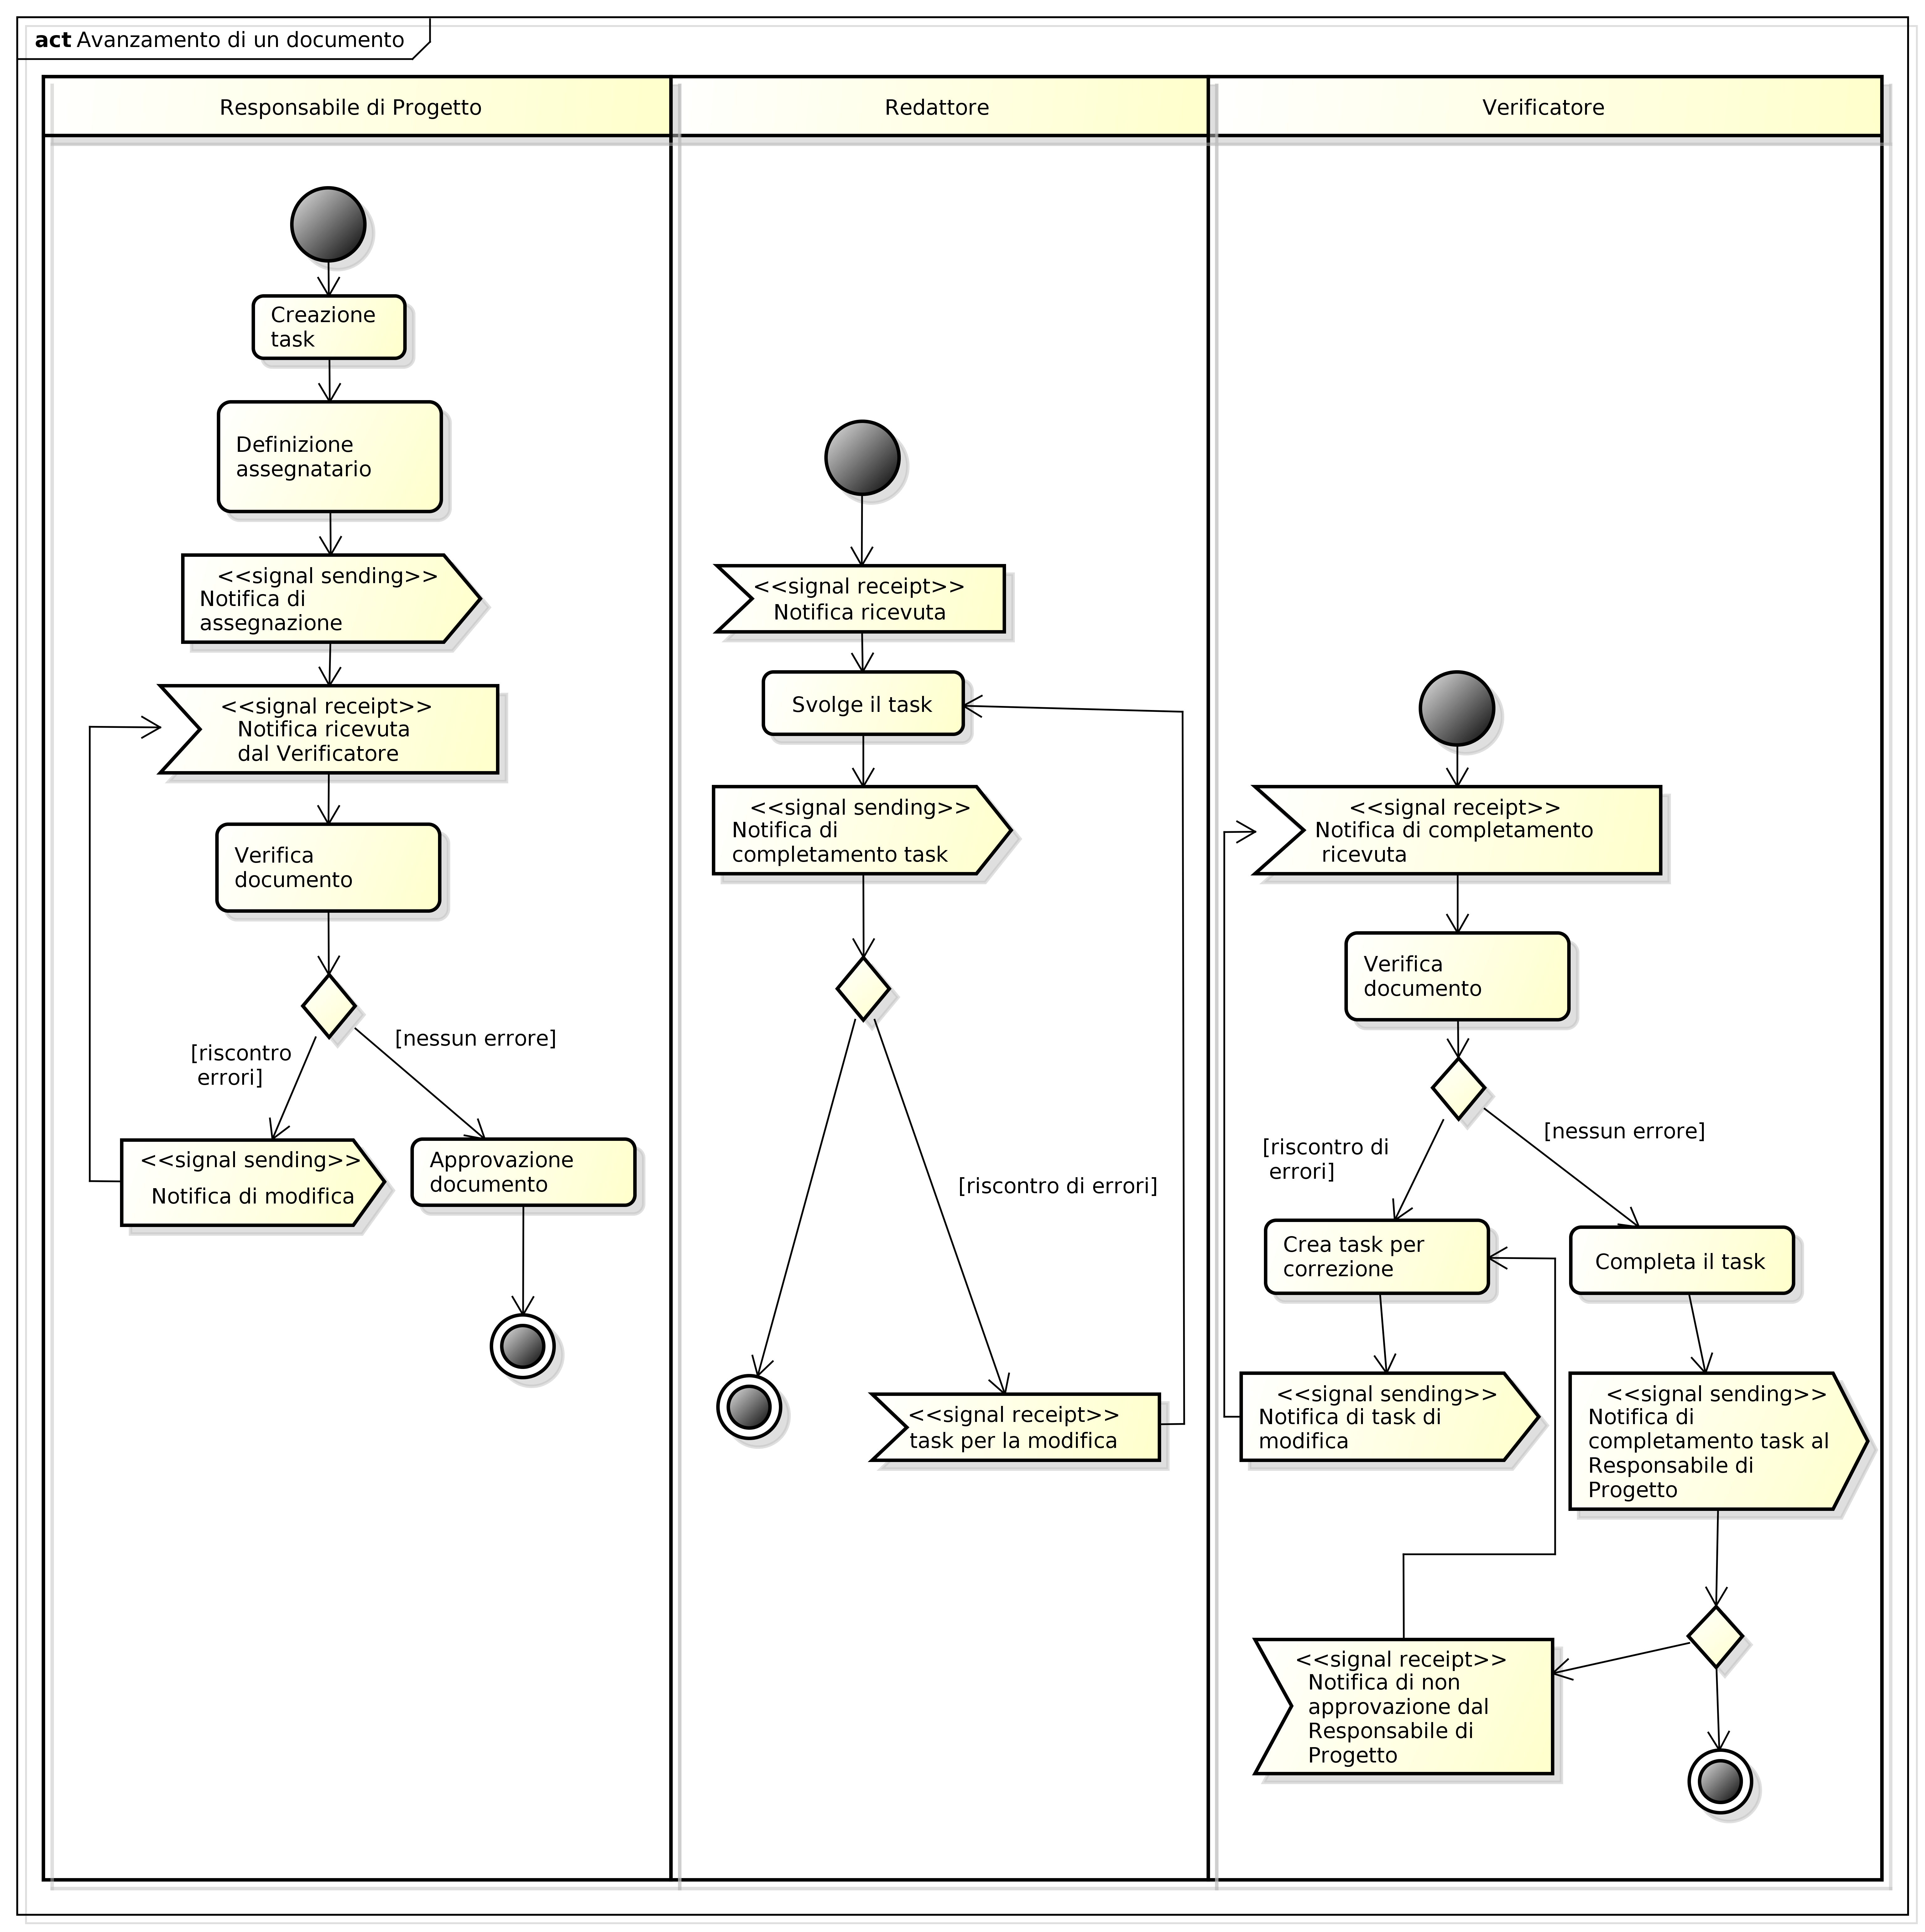
\includegraphics[scale=0.4]{immagini/avanzamento_documento.png}
\captionsetup{labelfont=bf}
\caption{Diagramma di attività - Avanzamento di un documento}\label{sec:Figura3}
\end{figure}

\subsubsection{Gestione del glossario}
Il popolamento del \textit{Glossario v1.0.0} è un'attività, mostrata in \hyperref[sec:Figura4]{Figura 4}, che coinvolge redattori e \textit{Verificatori}, e si svolge come segue:
\begin{itemize}
	\item [1.] {\textbf{Individuazione di un nuovo termine}}: se durante la stesura di un documento il redattore identifica un nuovo termine che ritiene debba essere inserito nel \textit{Glossario v1.0.0}, è tenuto a trascriverlo all'interno di un apposito documento (Glossario Provvisorio) presente nella sezione \textit{Notebooks}\G\ di Teamwork\G.
	\item [2.] {\textbf{Inserimento del termine nel Glossario}}: un \textit{Verificatore} deve occuparsi dell'approvazione di un dato termine presente in Glossario Provvisorio di Teamwork e dell'inserimento dello stesso all'interno del \textit{Glossario v1.0.0}. Una volta inserito, il termine deve essere rimosso dal documento su Teamwork.
\end{itemize}
 Nei documenti, il pedice \G\ appare solamente alla prima occorrenza del vocabolo all'interno di un paragrafo.

\begin{figure}[htbp]
\centering
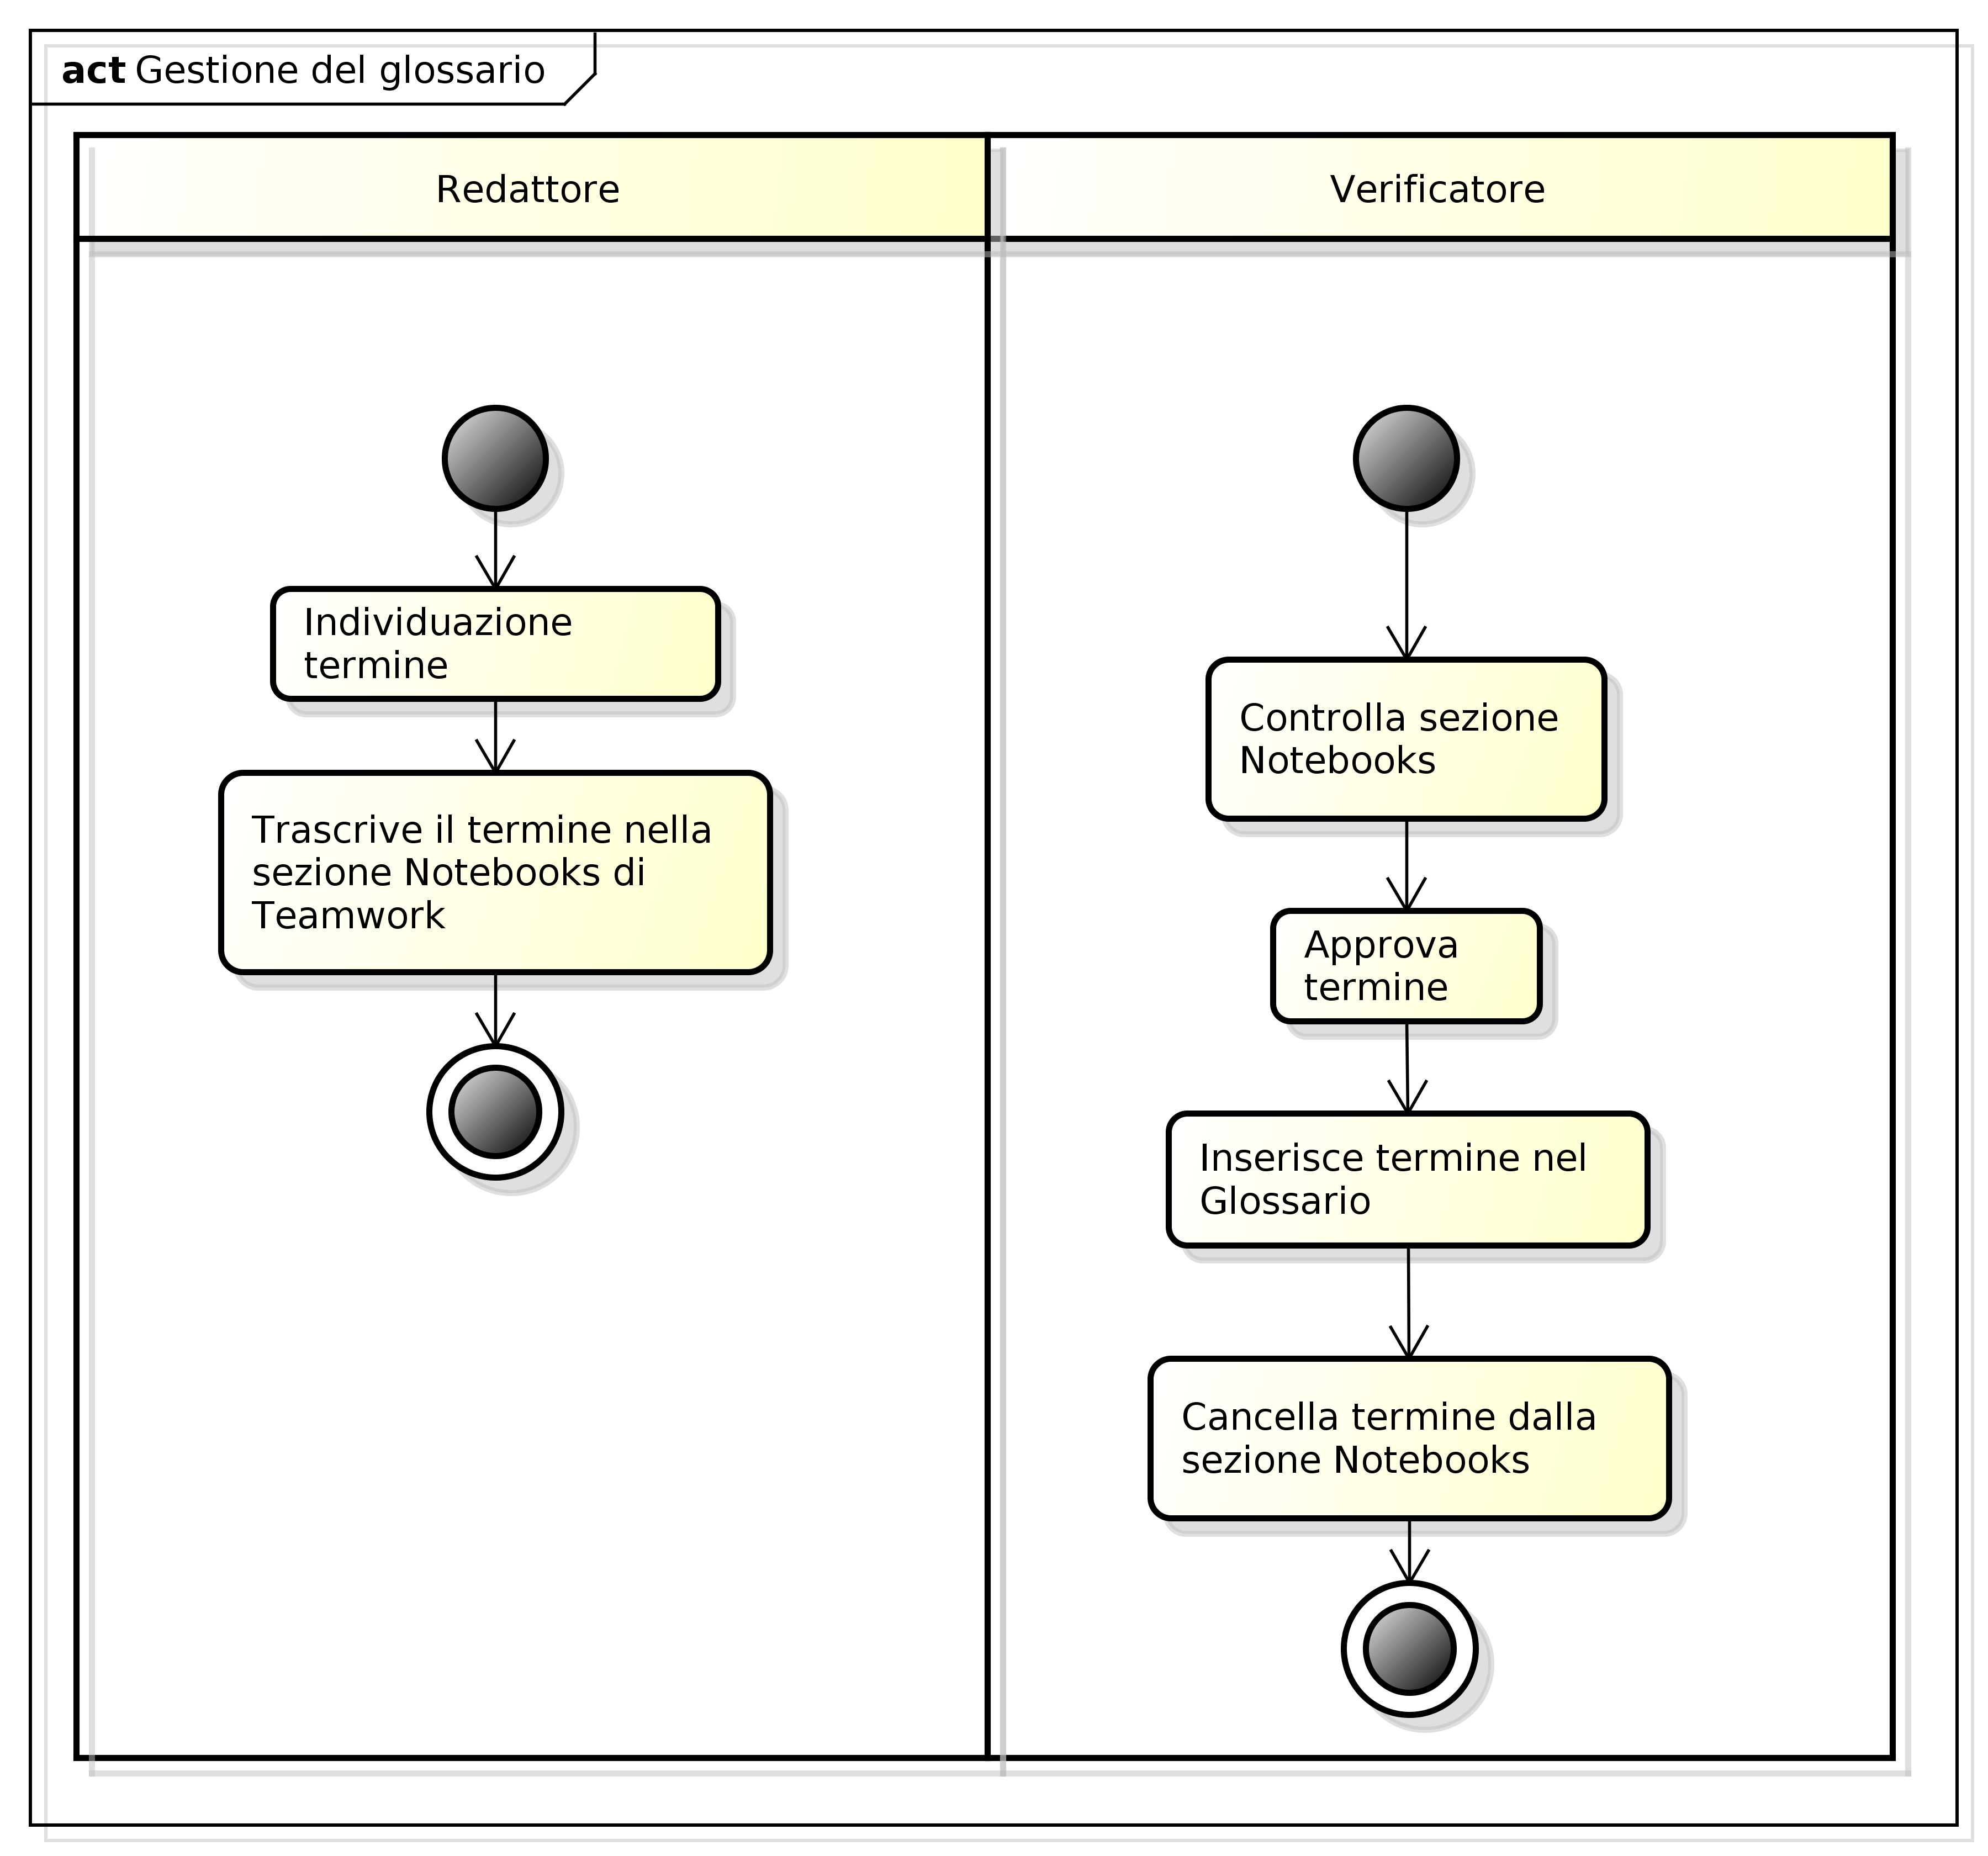
\includegraphics[scale=0.5]{immagini/gestione_glossario.png}
\captionsetup{labelfont=bf}
\caption{Diagramma di attività - Gestione del Glossario}\label{sec:Figura4}
\end{figure}

\subsubsection{Norme}
\paragraph{Progettazione e sviluppo dei documenti}
Ogni documento deve rispettare in modo assoluto la seguente serie di norme.

\paragraph{Versionamento}
\label{sec:versionamento}
Ogni documento prodotto deve essere corredato dal numero di versione. Il formato adottato è
il seguente:
\begin{center}
	vX.Y.Z
\end{center}
tale che:
\begin{itemize}
	\item{\textbf{X}}: indice di versione principale. Tale valore viene incrementato ad ogni approvazione del documento e ne indica la versione di rilascio;
	\item{\textbf{Y}}: indice di modifica parziale. Tale valore viene incrementato ad ogni verifica del documento;
	\item{\textbf{Z}}: indice di modifica minore. Tale valore viene incrementato ad ogni cambiamento che avviene nel documento.
\end{itemize}

\paragraph{Template}
La creazione dei documenti avviene attraverso l'utilizzo di un \textit{template}\G\ sviluppato con \LaTeX\ e la cui struttura \textbf{non} deve essere modificata a meno di direttive imposte dal \textit{Responsabile di Progetto}. Il \textit{template} funge da supporto per la stesura organizzata e sistematica dei documenti e, grazie ad esso, ogni componente del documento ha una precisa impostazione che non può essere modificata o equivocata dai redattori.

\paragraph{Struttura dei documenti}
L'organizzazione dei documenti è la seguente: 
\begin{itemize}
	\item Vi è una cartella generale in cui sono contenuti il \textit{template}\G\ \LaTeX\ e le varie cartelle specifiche di ogni documento;
	\item Nella cartella denominata "\textit{template}" sono contenuti i \textit{file} di configurazione e strutturazione del \textit{template}. Il contenuto della cartella non deve essere modificato, previa autorizzazione da parte del \textit{Responsabile di Progetto};
	\item Nella cartella specifica di ogni documento è presente un \textit{file} di tipo nome\_documento.tex, tramite cui si determina la struttura dello specifico documento. Inoltre è presente una sotto cartella "sezioni" contenente le varie sezioni nelle quali sono scritti i contenuti veri e propri.
\end{itemize}

\subparagraph{Prima pagina}
\label{sec:primaPagina}
Nella prima pagina sono presenti tutte le informazioni generali relative al documento:
\begin{itemize}
	\item Nome del progetto;
	\item Logo del gruppo;
	\item Nome del documento;
	\item Versione del documento;
	\item Membri del gruppo che hanno lavorato come redattori, \textit{Verificatori} e \textit{Responsabili} per la stesura del documento. I nomi vanno scritti nel formato Nome Cognome;
	\item Specifica dell'uso del documento (interno o esterno);
	\item Lista di distribuzione del documento. I nomi vanno scritti nel formato Nome Cognome;
	\item Breve descrizione che precisa lo scopo del documento.
\end{itemize}
\subparagraph{Registro delle modifiche}
Nella seconda pagina si trova una tabella con il registro delle modifiche effettuate al documento. Esso è indispensabile per un corretto tracciamento delle varie fasi che si sono percorse lungo la stesura. Ogni riga corrisponde a una modifica dove vengono segnalati:
\begin{itemize}
	\item Descrizione dell'azione compiuta sul documento;
	\item Nome e cognome dell'autore della modifica;
	\item Data della modifica;
	\item Versione del documento a seguito della modifica.
\end{itemize}

\subparagraph{Indici}
In terza pagina è presente l'indice che tiene traccia delle varie sezioni in cui è stato suddiviso il documento. La profondità dell'indice arriva fino a cinque livelli: gli argomenti trattati sono suddivisi in sezioni, sottosezioni, sotto-sottosezioni, paragrafi e sotto-paragrafi.
Se sono presenti immagini e/o tabelle, viene stilato in automatico un indice che ne tiene traccia.
\subparagraph{Formattazione di una pagina}
Tutte le pagine dei documenti seguono una precisa formattazione imposta dal \textit{template}\G :
\begin{itemize}
	\item{\textbf{Intestazione}}: contiene sulla sinistra il logo del gruppo e sulla destra il nome della sezione in cui è contenuta la pagina;
	\item{\textbf{Contenuto}}: contiene il contenuto effettivo della pagina le cui norme tipografiche sono descritte in \hyperref[sec:normeTipografiche]{3.1.4.5.6 Norme Tipografiche};
	\item{\textbf{Piè di pagina}}: contiene sulla sinistra il nome del documento con relativo numero di versione e sulla destra il numero della pagina, scritto nel formato "X di Y", con X numero di pagina corrente e Y numero delle pagine totali.
\end{itemize}
La suddetta struttura si ripete per ogni pagina ad eccezione della prima, il cui formato è descritto in \hyperref[sec:primaPagina]{3.1.4.4.1 Prima Pagina}.

\paragraph{Suddivisione dei documenti}
\label{sec:suddivisioneDocumenti}
\subparagraph{Norme di Progetto}
Il documento ha lo scopo di definire le linee guida per le varie attività di sviluppo. Al suo interno sono raccolte le norme, le procedure e gli strumenti che il gruppo adotterà nel corso della realizzazione del progetto. Il documento è destinato a uso interno.
\subparagraph{Studio di Fattibilità}
Il documento ha lo scopo di descrivere le considerazioni elaborate dal gruppo per l'accettazione del progetto che si è deciso di prendere in carico, con valutazione di rischi, costi e benefici calcolati sulla base di una prima analisi del capitolato. Al suo interno vengono motivate le scelte che hanno spinto il gruppo all'esclusione degli altri progetti. Il documento è destinato a uso interno.
\subparagraph{Analisi dei Requisiti}
Il documento ha lo scopo di identificare e descrivere i requisiti, i vincoli e gli obiettivi necessari allo sviluppo del progetto. Al suo interno sono contenuti i casi d'uso e i requisiti utili alla realizzazione del progetto, accompagnati da diagrammi e grafici di interazione fra utenti e sistema. Il documento è destinato a uso esterno.
\subparagraph{Piano di Progetto}
Il documento ha lo scopo di pianificare lo svolgimento del progetto. Al suo interno sono fissate le risorse disponibili, la suddivisione e il calendario delle attività, e gli obiettivi necessari per valutare in modo corretto il grado di avanzamento dello sviluppo. Il documento è destinato a uso esterno.
\subparagraph{Piano di Qualifica}
Il documento ha lo scopo di spiegare le strategie applicate al progetto per ottenere gli obiettivi di qualità. Al suo interno sono presenti le attività di verifica e pianificazione con i relativi test da sviluppare. Il documento è destinato a uso esterno.
\subparagraph{Specifica Tecnica}
Il documento ha lo scopo di descrivere l'architettura logica del progetto, senza fissare i dettagli implementativi, ma definendo linee e strategie di realizzazione, al fine di stabilire cause ed effetti e avere una visione complessiva della soluzione. Al suo interno è contenuta una prima progettazione ad alto livello del sistema da sviluppare. In esso vengono specificati i \textit{design pattern}\G\ utilizzati. Il documento è destinato a uso esterno. 
\subparagraph{Definizione di Prodotto}
Il documento ha lo scopo di descrivere nel dettaglio l'architettura del prodotto da sviluppare. Il suo contenuto viene utilizzato dai \textit{Programmatori} per sviluppare il \textit{software}. Il documento è destinato a uso esterno.
\subparagraph{Glossario}
Il documento ha lo scopo di raccogliere, in ordine alfabetico, tutti i termini ambigui presenti nei documenti accompagnati da una loro definizione. Il documento è destinato a uso esterno.

\paragraph{Norme tipografiche}
\label{sec:normeTipografiche}
Al fine di rendere omogenea e coesa la stesura dei documenti, il contenuto deve rispettare le seguenti norme tipografiche.
\subparagraph{Stile del testo}
\begin{itemize}
\item \textbf{Corsivo}: va utilizzato tassativamente per indicare termini in lingua inglese che non fanno parte dell'uso comune dell'italiano, citazioni, nomi di documenti interni, ruoli ufficiali dei membri del gruppo ed eventualmente (ma con moderazione) per parole che si ritiene debbano essere messe in risalto rispetto al resto del testo; 
\item \textbf{Grassetto}: va usato per evidenziare parole significative di estrema importanza. È necessario che non se ne abusi. Viene applicato automaticamente a titoli di sezioni, sottosezioni e paragrafi. Viene utilizzato negli elenchi puntati per evidenziare un termine seguito da una descrizione;
\item \textbf{Maiuscolo}: viene utilizzato per scrivere acronimi e macro \LaTeX. Inoltre, lettere maiuscole vengono usate per riferirsi ai ruoli di progetto, alle fasi di lavoro e ai seguenti nomi: del \textit{team}, del progetto e dei documenti;
\item \LaTeX: viene usato il comando \textbackslash LaTeX per ogni occorrenza del termine \LaTeX;
\item \textbf{Font}: nel \textit{template} è impostato Gillius, un \textit{font} professionale di tipo \textit{sans-serif} il cui scopo è garantire maggiore leggibilità del testo su schermo;
\item \textbf{Monospace}\G: tipologia di font che serve per formattare correttamente il testo contenente porzioni di codice, comandi e indirizzi \textit{web}.
\end{itemize}
\subparagraph{Punteggiatura}
\begin{itemize}
\item \textbf{Spaziatura}: lo spazio non può mai precedere un carattere di punteggiatura.
\end{itemize} 
\subparagraph{Composizione del testo}
\begin{itemize}
	\item {\textbf{Elenchi puntati}}: l’ultima voce deve terminare con un punto, mentre le altre con un punto e virgola. La prima lettera di ogni punto va scritta in maiuscolo e la prima parola va in grassetto se seguita da una descrizione della stessa. Gli elenchi numerati vengono utilizzati per descrivere sequenze di azioni ordinate;
	\item \textbf{Pedice G}: il pedice \G\ è utilizzato al solo scopo di indicare termini potenzialmente ambigui che si possono reperire nel documento \textit{Glossario v1.0.0}.
\end{itemize}

\subparagraph{Formati} Elenco dei formati rispettati dai documenti:
\begin{itemize}
	\item \textbf{Data}: il formato utilizzato è dd/mm/yyyy. Per esempio, 16/11/2004 indica il 16 novembre 2004;
	\item \textbf{Ora}: si utilizza il formato internazionale previsto dalla norma ISO 8601 del tipo [hh]:[mm]:[ss] ove [hh] indica l'ora, [mm] i minuti, [ss] i secondi, espressi con due cifre. Ad esempio, 18:35:26 indica le ore 18, 35 minuti e 26 secondi; 04:09:01 indica le ore 4, 9 minuti e 1 secondo;
	\item \textbf{Percorsi}: viene utilizzato il separatore \textit{slash} (/) per indicare il percorso di un \textit{file}. Per esempio, cartella1/cartella2/file\_esempio.txt;
	\item \textbf{Nomi di persona}: espressi nel formato Nome Cognome.
\end{itemize}

\subparagraph{Sigle} Elenco delle sigle che possono apparire nel corso dei documenti:
\begin{itemize}
	\item \textbf{AdR}: Analisi dei Requisti; 
	\item \textbf{GL}: Glossario; 
	\item \textbf{NdP}: Norme di Progetto; 
	\item \textbf{PdP}: Piano di Progetto;
	\item \textbf{PdQ}: Piano di Qualifica; 
	\item \textbf{SdF}: Studio di Fattibilità;
	\item \textbf{ST}: Specifica Tecnica; 
	\item \textbf{RA}: Revisione di Accettazione;
	\item \textbf{RP}: Revisione di Progettazione;
	\item \textbf{RQ}: Revisione di Qualifica;
	\item \textbf{RR}: Revisione dei Requisiti.
\end{itemize}

\paragraph{Componenti grafiche}
\subparagraph{Immagini e diagrammi}
Tutte le immagini (diagrammi inclusi) da inserire nei documenti devono essere salvate in formato \textit{Portable Network Graphics} (PNG\G) o \textit{Portable Document Format} (PDF\G). Immagini e diagrammi vanno inserite nella cartella "immagini" relativa al documento specifico.

\subsection{Processo di verifica e validazione}
Il processo di verifica consiste nel controllare che il materiale prodotto al raggiungimento delle \textit{milestone}\G\ sia conforme agli obiettivi prefissati. Pertanto, è necessario verificare che non siano stati commessi errori. Il prodotto è validato se il risultato ottenuto è consistente e conforme alle attese. Una corretta applicazione del processo di verifica genera un aumento del rapporto fra efficienza ed efficacia, riducendo il tempo impiegato nel percorso di analisi e correzione.
\subsubsection{Attività}
\paragraph{Analisi statica}
L'attività di analisi statica è una tecnica di verifica applicabile sia a documenti che a codice sorgente che va ad analizzare il solo testo del \textit{file} senza mandarlo in esecuzione. Tale tecnica viene utilizzata durante l'intero sviluppo del progetto e si pone come obiettivo il ritrovamento di eventuali anomalie. I metodi di controllo sono i seguenti:
\begin{itemize}
	\item \textbf{Walktrough}: si ricercano all'interno di testo o codice tutte le possibili anomalie; l'attività è eseguita da persone. L'analisi si basa sulla lettura di tutto il contenuto del \textit{file}. In seguito al ritrovamento di anomalie, le si analizza con il redattore del documento (o \textit{Programmatore} nel caso di codice) e si indaga per raggiungere una soluzione del problema. Tale tecnica risulta utile durante le prime fasi di sviluppo del progetto, in quanto manca, ai componenti, una visione complessiva del documento o del codice che si sta scrivendo. Permette così ai \textit{Verificatori}, dopo aver svolto le prime correzioni, di preparare una \textit{lista di controllo} con gli errori più frequenti in modo da migliorare l'efficienza delle verifiche future. A questo punto è possibile implementare un'analisi mirata e più efficiente attraverso il metodo dell'\textit{Inspection}.
	\item \textbf{Inspection}: si ricercano all'interno di un testo errori specifici; l'attività può essere eseguita sia da un umano che, nel caso di anomalie nella sintassi, da uno script. Il metodo focalizza la ricerca su errori presupposti identificati dalla \textit{lista di controllo}.
\end{itemize}
\paragraph{Analisi dinamica}
L'attività di analisi dinamica è una tecnica di verifica applicabile solamente al \textit{software}. Tale tecnica può essere utilizzata per analizzare l'intero \textit{software} o una porzione limitata dello stesso. L'attività consiste nell'esecuzione di \textit{test} automatici realizzati dal \textit{team}. Le verifiche devono essere effettuate su un insieme finito di casi, con valori di ingresso, uno stato iniziale e un esito decidibile. Tutti i \textit{test} producono risultati automatici che inviano notifiche sulla tipologia di problema individuato. Ogni \textit{test} è ripetibile, ossia applicabile durante l'intero ciclo di vita\G\ del \textit{software}. Le caratteristiche da rispettare sono le seguenti: 
\begin{itemize}
	\item \textbf{Ambiente}: è necessario riportare l'ambiente sia \textit{software} che \textit{hardware} in cui il sistema esegue il \textit{test}. Deve essere specificato lo stato iniziale del sistema; 
	\item \textbf{Specifica}: è necessario riportare i dati in ingresso e in uscita per verificare l'esito del \textit{test}, ossia se il codice analizzato è conforme alle aspettative;
	\item \textbf{Procedure}: è possibile specificare ulteriori istruzioni per l'esecuzione dei \textit{test}. Inoltre possono essere riportate istruzioni sulla corretta lettura dei risultati.
\end{itemize}
\paragraph{Gestione anomalie}
Se si dovessero riscontrare anomalie o discordanze normative durante le attività di verifica, il \textit{Verificatore} ha il dovere di notificarle all'assegnatario del \textit{task}\G.  

\paragraph{Tracciamento}
L'attività di tracciamento svolta dai \textit{Verificatori} consiste nella catalogazione di tutti i casi d'uso e dei requisiti che ne derivano ed evidenziare la corrispondenza fra di essi in modo da avere ben chiaro i processi di derivazione.

\subsubsection{Procedure}
\paragraph{Procedure di assegnazione delle anomalie}
L'assegnazione delle anomalie rilevate dai \textit{Verificatori} avviene attraverso l'uso del servizio \textit{web} Teamwork\G. Gli errori vanno gestiti attraverso \textit{task}\G\ da creare in una delle seguenti categorie:
\begin{itemize}
	\item \textbf{Anomalie Documenti}: gruppo di \textit{task} dedicato agli errori rilevati nella documentazione;
	\item \textbf{Anomalie Codice}: gruppo di \textit{task} dedicato agli errori rilevati nel codice.
\end{itemize}
I \textit{task} contenuti nei suddetti gruppi devono essere creati seguendo la seguente serie di azioni, mostrate anche in \hyperref[sec:Figura5]{Figura 5}:
\begin{itemize}
	\item [1.] Assegnazione di un titolo al nuovo \textit{task} contenente in testa la dicitura [BUG];
	\item [2.] Descrizione dettagliata dell'anomalia rilevata. Deve essere specificato il punto esatto del file in cui è stato individuato l'errore;
	\item [3.] Assegnazione del \textit{task} al membro del gruppo che ha commesso l'errore;
	\item [4.] Assegnazione di una data di scadenza per la correzione dell'errore.
\end{itemize} 
Una volta creato il \textit{task}, un'email viene inviata automatica all'assegnatario, che avrà l'incarico di risolvere il \textit{bug}\G\ entro la data di scadenza segnata. La priorità di risoluzione degli errori deve essere svolta secondo l'ordine di scadenza organizzato dal \textit{Responsabile di Progetto}.

\begin{figure}[htbp]
\centering
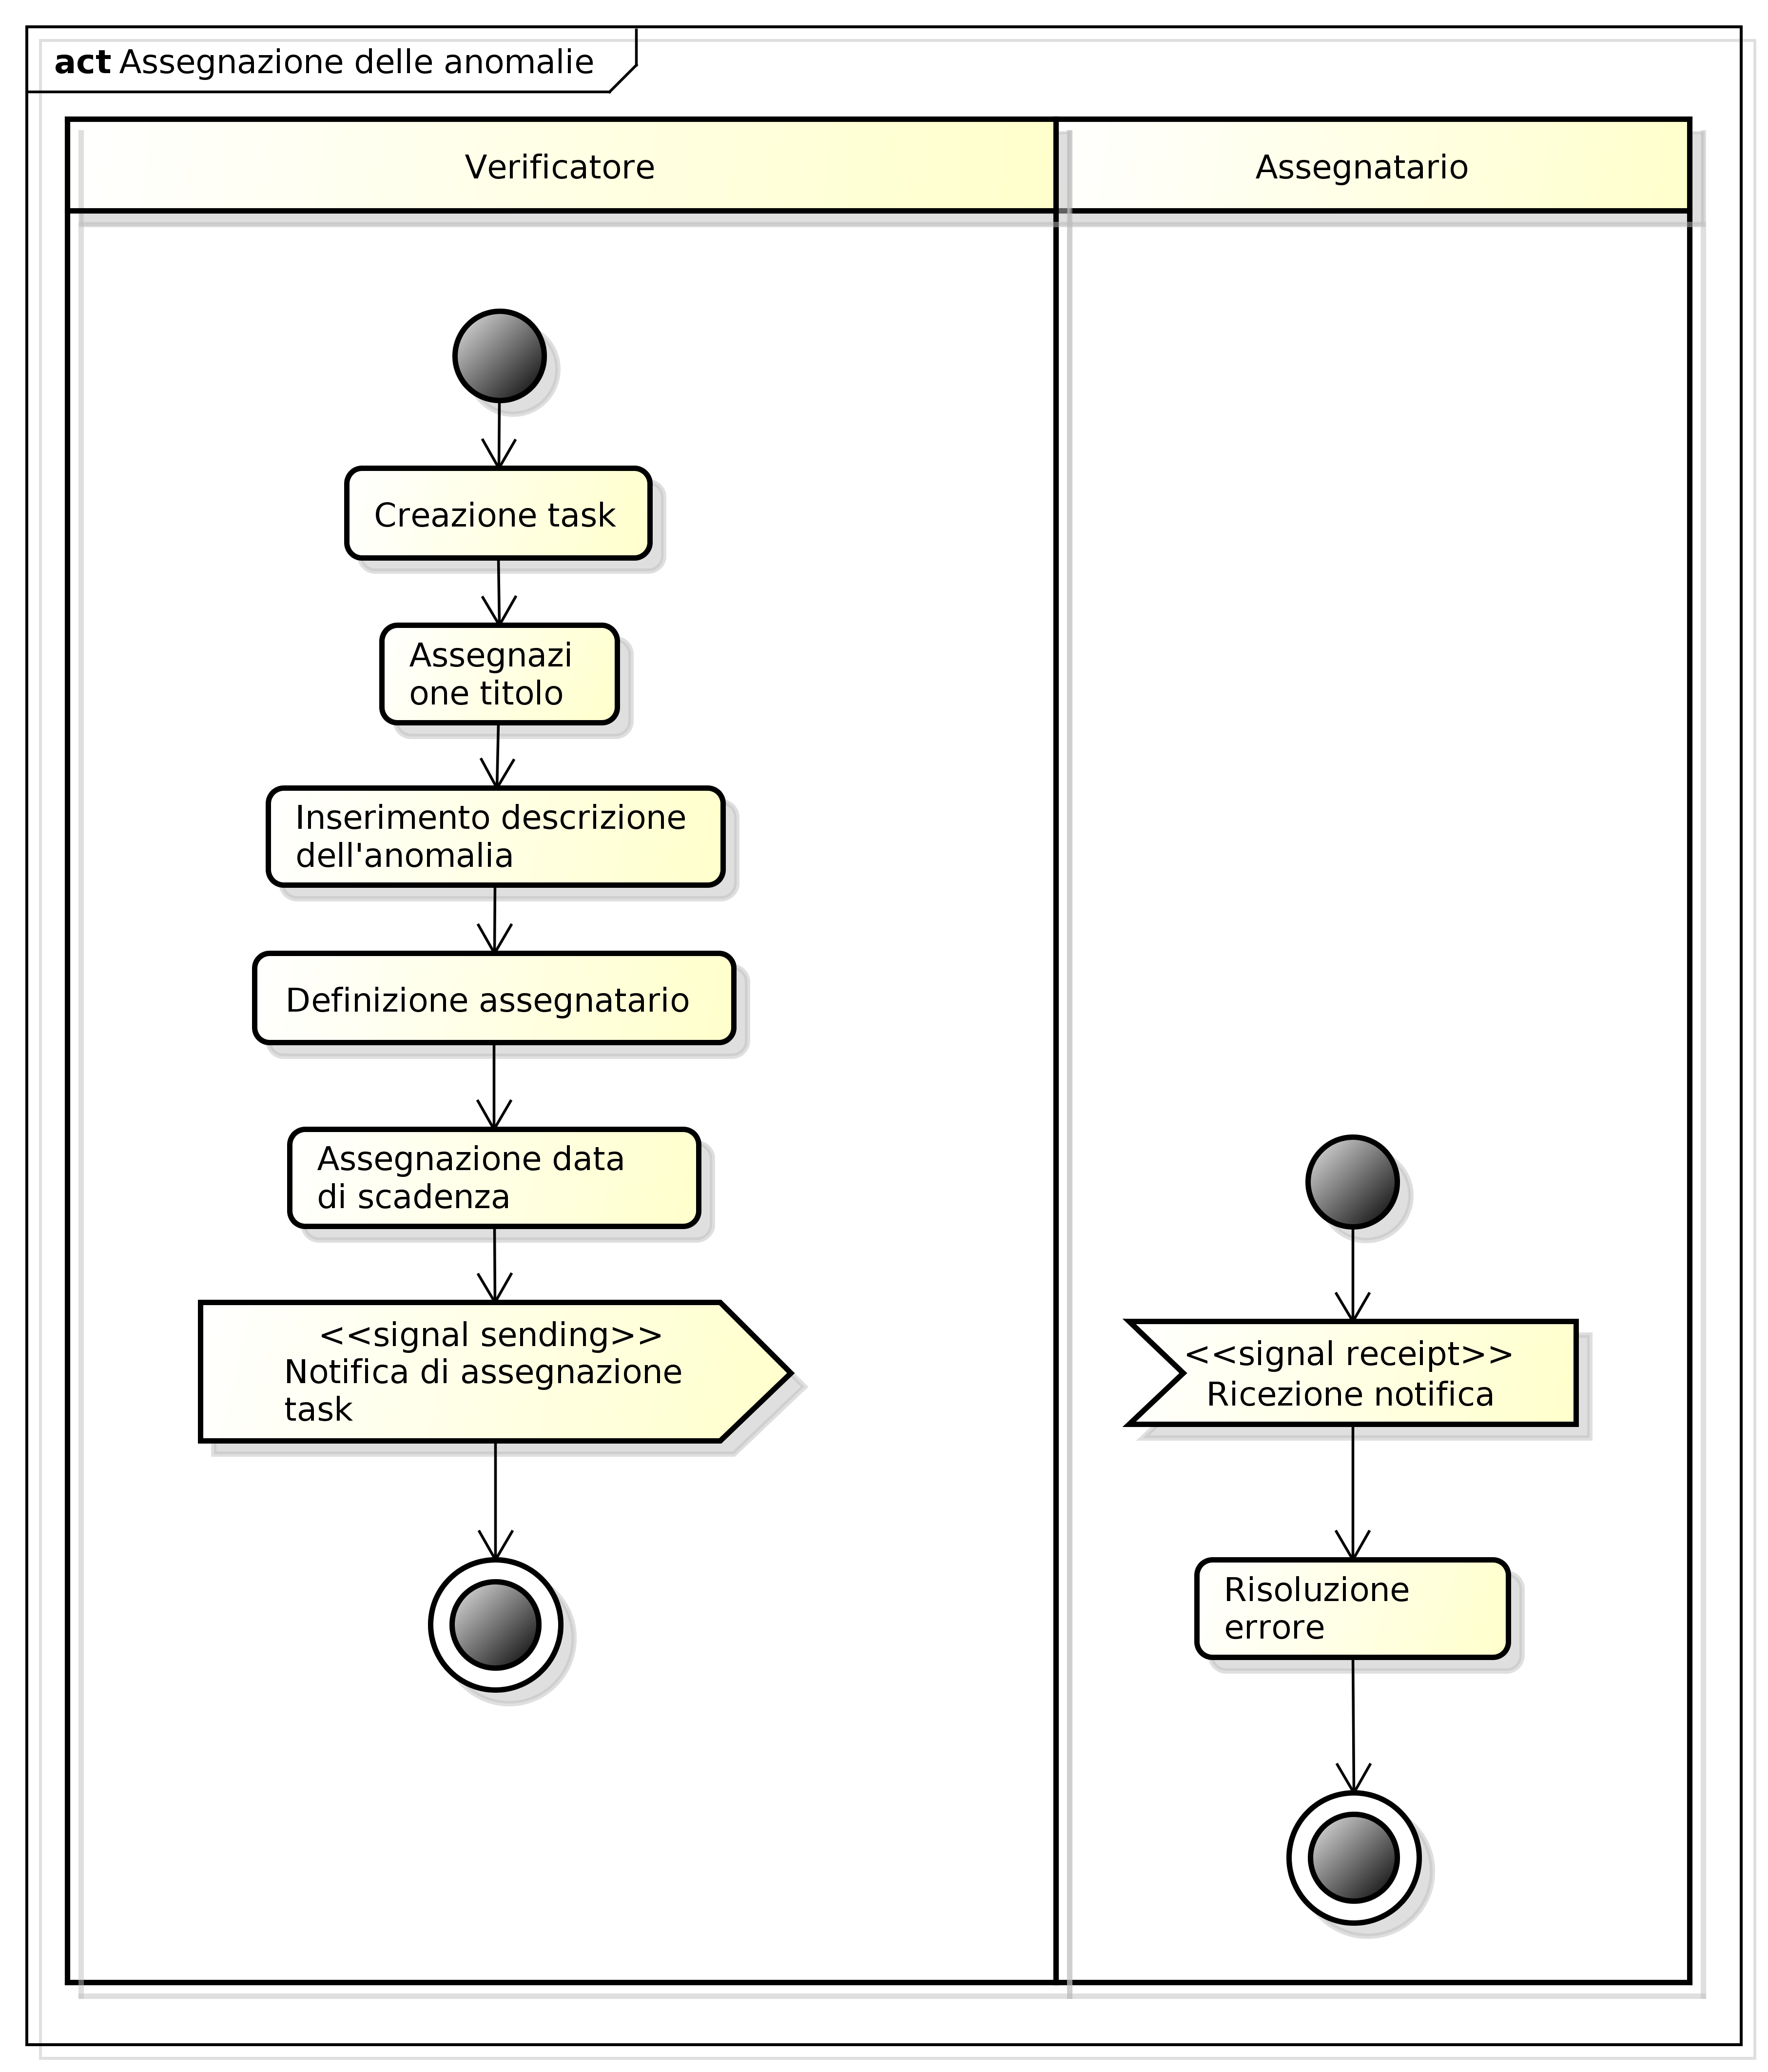
\includegraphics[scale=0.5]{immagini/assegnazione_anomalie.png}
\captionsetup{labelfont=bf}
\caption{Diagramma di attività - Procedura di assegnazione delle anomalie}\label{sec:Figura5}
\end{figure}

\subsubsection{Strumenti}
\paragraph{Correzione ortografica}
Come supporto alla correzione dei documenti si utilizza il correttore ortografico automatico incluso nell'\textit{editor} TeXstudio\G. Gli strumenti offerti da TeXstudio sono utili alla sola correzione di errori ortografici gravi, ma non è preciso per l'individuazione di errori più sottili. Un'analisi più approfondita spetta ai \textit{Verificatori}.
\paragraph{Calcolo dell'indice Gulpease}
Affinchè un documento possa superare la fase di accettazione, è necessario che soddisfi il test di leggibilità con un indice Gulpease\G\ superiore a 40 punti. Per maggiori dettagli si veda il documento \textit{Piano di Qualifica v1.0.0}.
\newpage